\documentclass[convert={density=300,size=1080x800,outext=.png}]{standalone}
\usepackage{tkz-graph}
\usetikzlibrary{arrows,positioning,shapes,shapes.multipart,patterns,mindmap,shadows}
\usepackage{xcolor}
\usepackage{helvet}
\renewcommand{\familydefault}{\sfdefault}


\begin{document}

\footnotesize
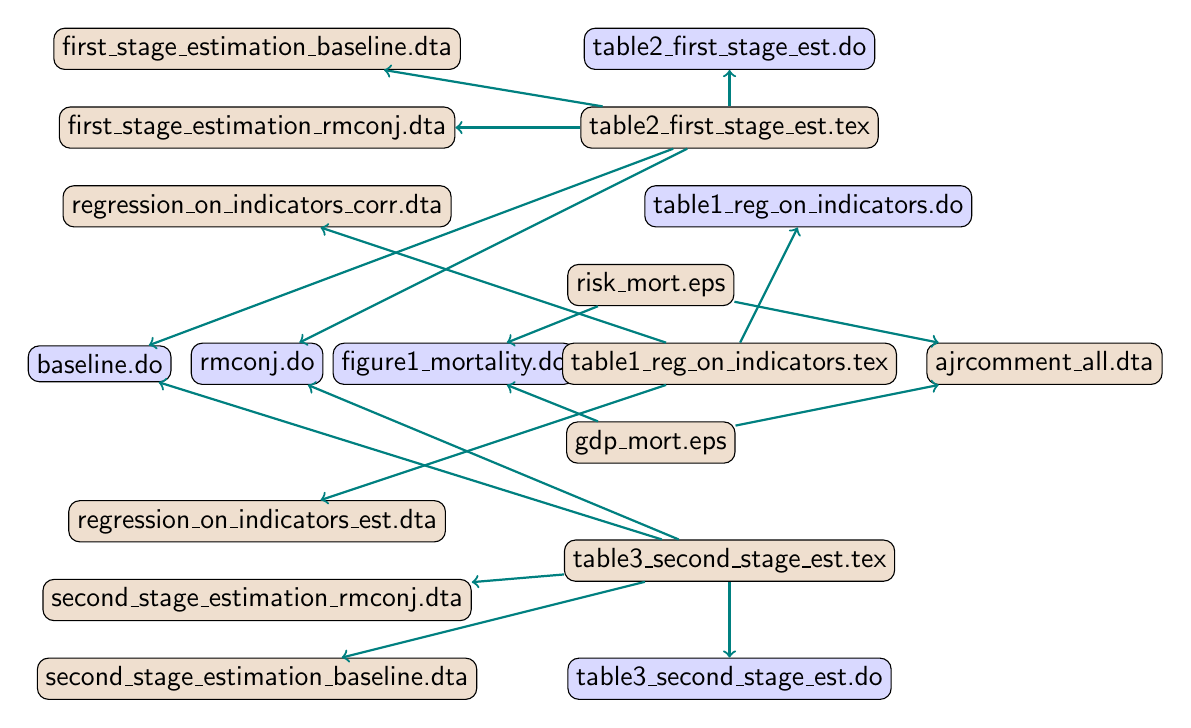
\begin{tikzpicture}[every node/.style={
    rectangle,
    rounded corners,
    inner sep=3pt,
    draw,
    fill=brown!25
}]
    \node (ajrcomment_all_dta) [shift={(19, 0)}]
    {
        ajrcomment\_all.dta
    };

    \node (baseline_do) [fill=blue!15, shift={(7, 0)}]
    {
        baseline.do
    };
    \node (rmconj_do) [fill=blue!15, shift={(9, 0)}]
    {
        rmconj.do
    };


    \node (regression_on_indicators_corr_dta) [shift={(9, 2)}]
    {
        regression\_on\_indicators\_corr.dta
    };

    \node (regression_on_indicators_est_dta) [shift={(9, -2)}]
    {
        regression\_on\_indicators\_est.dta
    };

    \node (first_stage_estimation_baseline_dta) [shift={(9, 4)}]
    {
        first\_stage\_estimation\_baseline.dta
    };

    \node (first_stage_estimation_rmconj_dta) [shift={(9, 3)}]
    {
        first\_stage\_estimation\_rmconj.dta
    };

    \node (second_stage_estimation_baseline_dta) [shift={(9, -4)}]
    {
        second\_stage\_estimation\_baseline.dta
    };

    \node (second_stage_estimation_rmconj_dta) [shift={(9, -3)}]
    {
        second\_stage\_estimation\_rmconj.dta
    };


    \node (figure1_mortality_do) [fill=blue!15, shift={(11.5, 0)}]
    {
        figure1\_mortality.do
    };

    \node (risk_mort_eps) [shift={(14, 1)}]
    {
        risk\_mort.eps
    };
    \node (gdp_mort_eps) [shift={(14, -1)}]
    {
        gdp\_mort.eps
    };

    \node (table1_reg_on_indicators_tex) [shift={(15, 0)}]
    {
        table1\_reg\_on\_indicators.tex
    };

    \node (table1_reg_on_indicators_do) [fill=blue!15, shift={(16, 2)}]
    {
        table1\_reg\_on\_indicators.do
    };


    \node (table2_first_stage_est_tex) [shift={(15, 3)}]
    {
        table2\_first\_stage\_est.tex
    };

    \node (table2_first_stage_est_do) [fill=blue!15, shift={(15, 4)}]
    {
        table2\_first\_stage\_est.do
    };

    \node (table3_second_stage_est_tex) [shift={(15, -2.5)}]
    {
        table3\_second\_stage\_est.tex
    };

    \node (table3_second_stage_est_do) [fill=blue!15, shift={(15, -4)}]
    {
        table3\_second\_stage\_est.do
    };

    \draw[->, teal, thick] (risk_mort_eps) to (ajrcomment_all_dta);
    \draw[->, teal, thick] (gdp_mort_eps) to (ajrcomment_all_dta);
    \draw[->, teal, thick] (risk_mort_eps) to (figure1_mortality_do);
    \draw[->, teal, thick] (gdp_mort_eps) to (figure1_mortality_do);
    \draw[->, teal, thick] (table1_reg_on_indicators_tex) to (regression_on_indicators_est_dta);
    \draw[->, teal, thick] (table1_reg_on_indicators_tex) to (regression_on_indicators_corr_dta);
    \draw[->, teal, thick] (table1_reg_on_indicators_tex) to (table1_reg_on_indicators_do);

    \draw[->, teal, thick] (table2_first_stage_est_tex) to (table2_first_stage_est_do);
    \draw[->, teal, thick] (table2_first_stage_est_tex) to (baseline_do);
    \draw[->, teal, thick] (table2_first_stage_est_tex) to (rmconj_do);
    \draw[->, teal, thick] (table2_first_stage_est_tex) to (first_stage_estimation_baseline_dta);
    \draw[->, teal, thick] (table2_first_stage_est_tex) to (first_stage_estimation_rmconj_dta);

    \draw[->, teal, thick] (table3_second_stage_est_tex) to (table3_second_stage_est_do);
    \draw[->, teal, thick] (table3_second_stage_est_tex) to (baseline_do);
    \draw[->, teal, thick] (table3_second_stage_est_tex) to (rmconj_do);
    \draw[->, teal, thick] (table3_second_stage_est_tex) to (second_stage_estimation_baseline_dta);
    \draw[->, teal, thick] (table3_second_stage_est_tex) to (second_stage_estimation_rmconj_dta);


\end{tikzpicture}

\end{document}

